\documentclass[aspectratio=169]{beamer}

\usetheme{Madrid}
\usecolortheme{seahorse}
\usepackage[utf8]{inputenc}
\usepackage[T1]{fontenc}
\usepackage{graphicx}
\usepackage{booktabs}
\usepackage{array}
\usepackage{xcolor}

\newcommand{\metricbox}[2]{%
  \begin{block}{#1}
    \centering\Large #2
  \end{block}
}

\title[US Housing Intelligence]{US Housing Market Analysis and Prediction}
\subtitle{Final Report, Streamlit App, Evaluation, Diagnostics, and OLAP Results}
\author{Ayoub Naouech \and Rayen Belhadj}
\institute{IT Business School -- Data Mining and Machine Learning}
\date{Academic Year 2025--2026}

\begin{document}

\begin{frame}
  \titlepage
\end{frame}

\begin{frame}{Presentation Roadmap}
\begin{enumerate}
  \item Project context and research objective
  \item Dataset, preparation, and methodology
  \item Streamlit app modules and screenshots
  \item Evaluation, diagnostics, OLAP, and paper-review results
  \item Limitations, future work, and final conclusion
\end{enumerate}
\end{frame}

\begin{frame}{Project Context}
\begin{itemize}
  \item The U.S. housing market is connected to household wealth, credit conditions, construction, inflation, and labor-market stability.
  \item Housing prices do not move because of one variable only; they react to demand, supply, rates, income, expectations, and market timing.
  \item The project transforms a housing and macroeconomic dataset into an interactive analytical platform.
  \item The final deliverables are the Streamlit app, the LaTeX report, the poster, and this presentation.
\end{itemize}
\end{frame}

\begin{frame}{Problem Statement}
\begin{block}{Main research question}
How can data mining and machine learning techniques be used to analyze and predict U.S. housing-market trends using macroeconomic indicators?
\end{block}
\begin{itemize}
  \item Identify useful variables for explaining the Home Price Index.
  \item Compare model performance using reproducible metrics.
  \item Make results understandable through visualizations and dashboard pages.
  \item Connect the technical results to real-estate theory and real market interpretation.
\end{itemize}
\end{frame}

\begin{frame}{Project Objective}
\begin{itemize}
  \item Analyze and predict U.S. housing-market behavior using data mining and machine learning.
  \item Use \texttt{Home\_Price\_Index} as the main target variable.
  \item Connect macroeconomic indicators, predictive models, OLAP segmentation, and housing-market theory.
  \item Deliver a final Streamlit dashboard that supports interpretation, reporting, and decision support.
\end{itemize}
\end{frame}

\begin{frame}{Dataset Overview}
\begin{columns}
\column{0.33\textwidth}
\metricbox{Rows}{242}
\column{0.33\textwidth}
\metricbox{Columns}{27}
\column{0.33\textwidth}
\metricbox{Period}{2004--2024}
\end{columns}
\vspace{0.6em}
\begin{itemize}
  \item The dataset combines housing-price information with macroeconomic indicators.
  \item Main columns include \texttt{Home\_Price\_Index}, \texttt{Mortgage\_Rate}, \texttt{Interest\_Rate}, \texttt{Unemployment\_Rate}, \texttt{Inflation\_CPI}, \texttt{Building\_Permits}, and \texttt{Median\_Income}.
\end{itemize}
\end{frame}

\begin{frame}{Methodology}
\begin{itemize}
  \item The project follows CRISP-DM: business understanding, data understanding, data preparation, modeling, evaluation, and deployment.
  \item The modeling workflow uses a chronological 80/20 train-test split to respect time order.
  \item The report combines model metrics with diagnostics, OLAP summaries, and paper-review interpretation.
  \item The Streamlit app makes the workflow interactive for users and evaluators.
\end{itemize}
\end{frame}

\begin{frame}{System Architecture}
\begin{columns}
\column{0.56\textwidth}
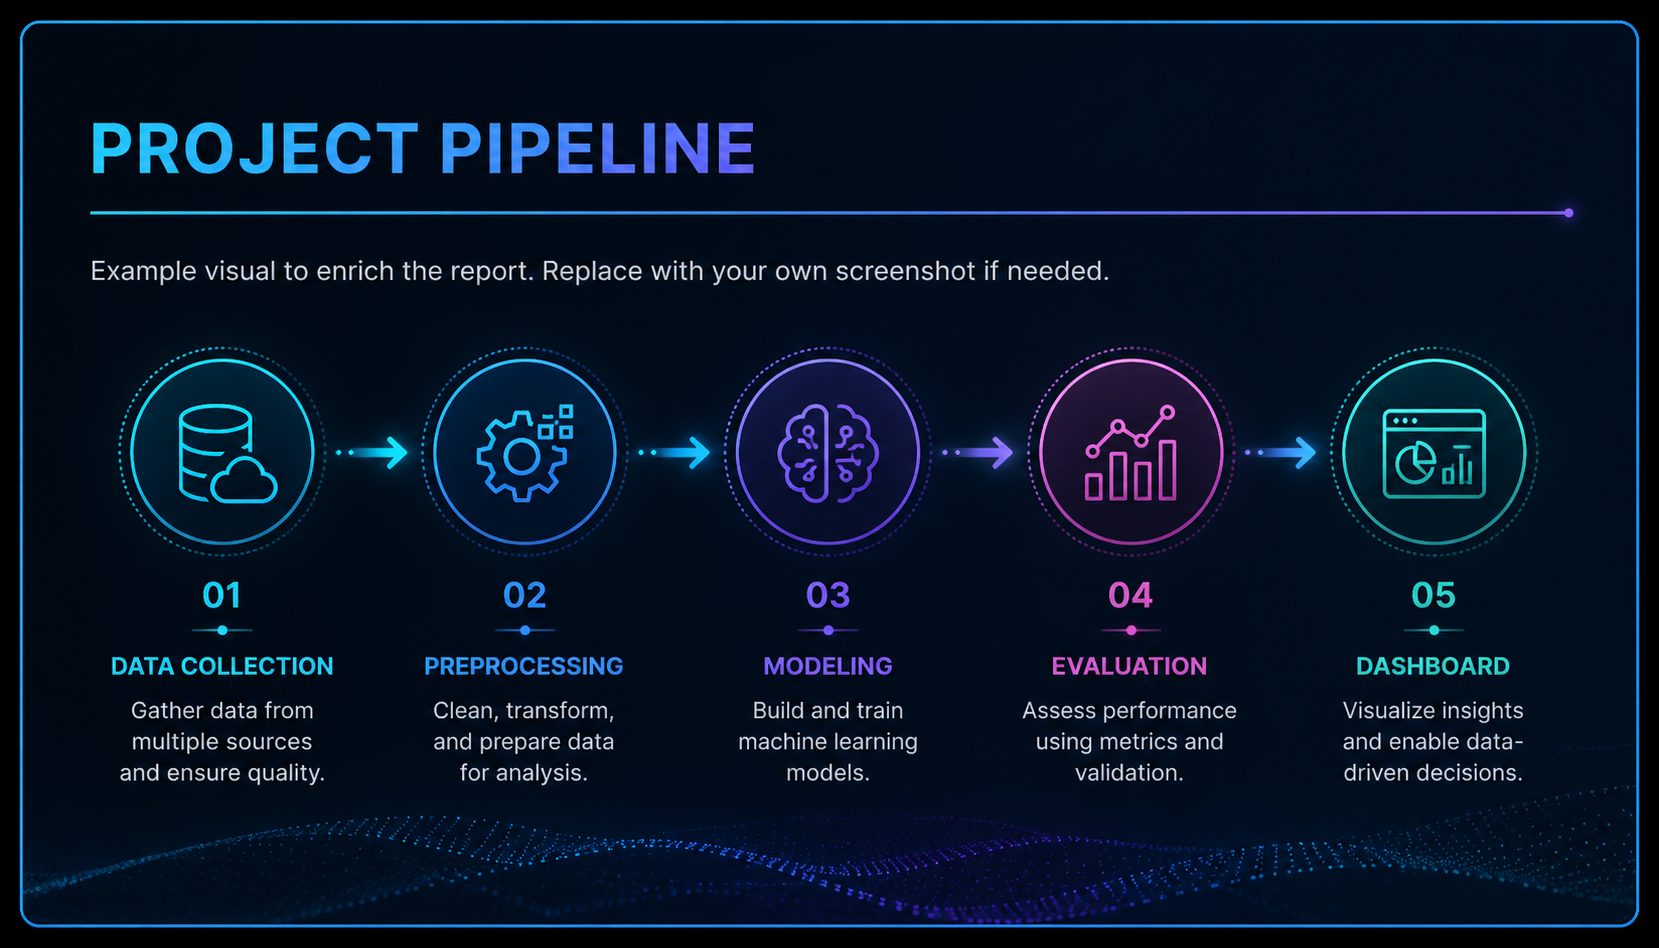
\includegraphics[width=\textwidth]{figures/project_pipeline.png}
\column{0.42\textwidth}
\begin{itemize}
  \item Data loading and cleaning
  \item Feature engineering
  \item EDA and visualization
  \item ML evaluation and diagnostics
  \item OLAP, export, paper review, and governance
\end{itemize}
\end{columns}
\end{frame}

\begin{frame}{Streamlit App Home}
\centering
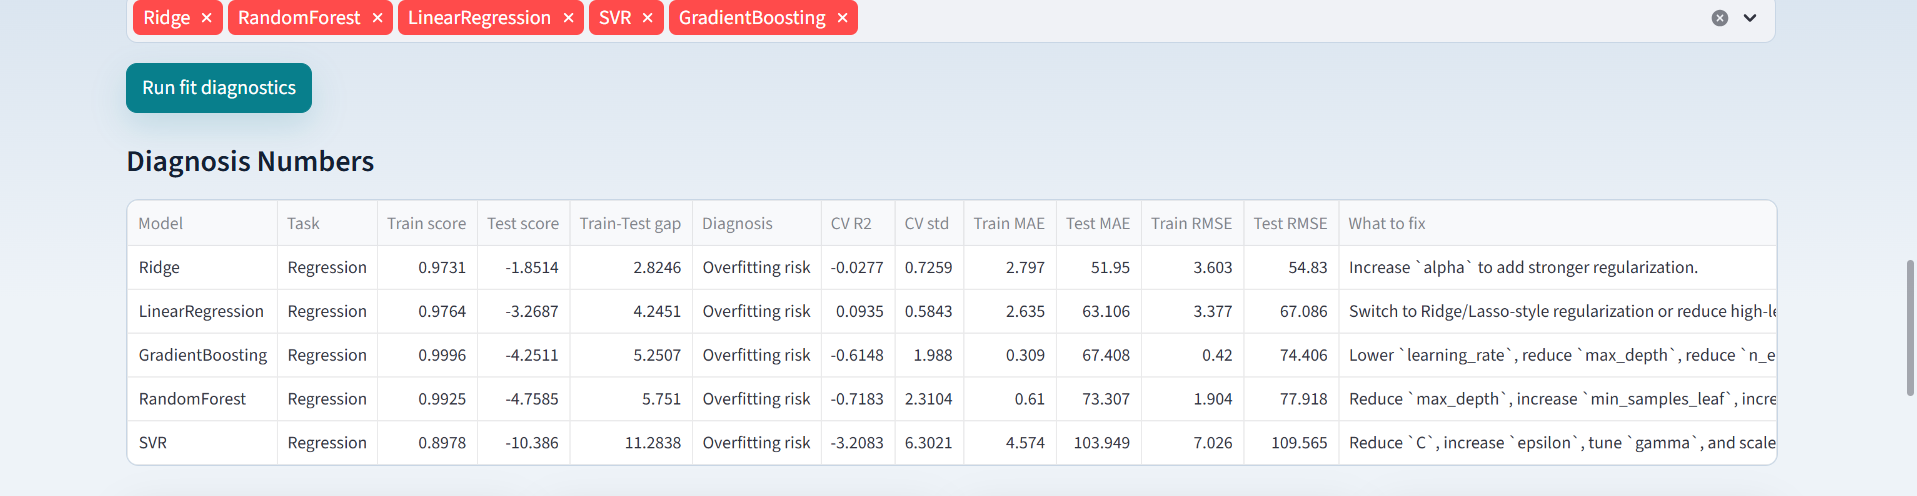
\includegraphics[height=0.78\textheight]{app_screenshots/app_home.png}
\end{frame}

\begin{frame}{Modeling Page In The App}
\centering
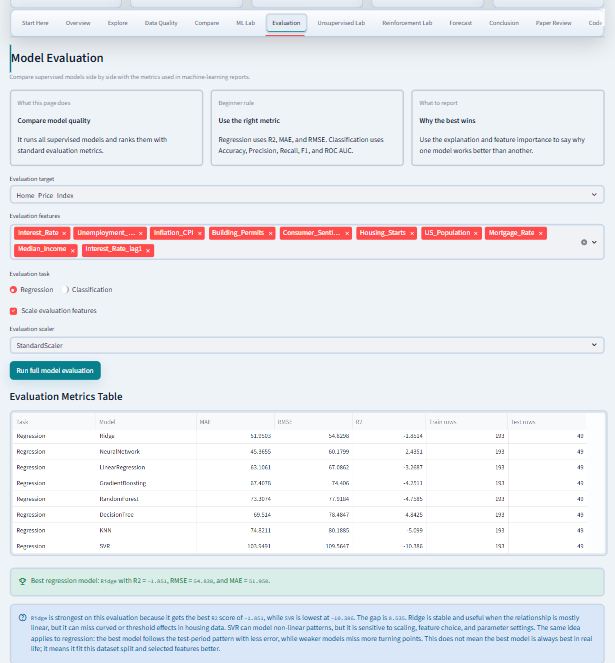
\includegraphics[height=0.78\textheight]{app_screenshots/app_modeling.png}
\end{frame}

\begin{frame}{Evaluation Page In The App}
\centering
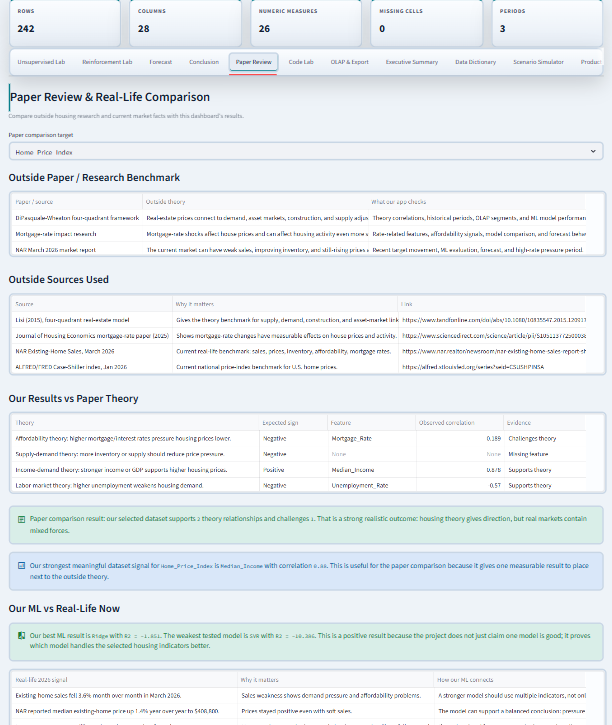
\includegraphics[height=0.78\textheight]{app_screenshots/app_evaluation.png}
\end{frame}

\begin{frame}{OLAP And Export Page}
\centering
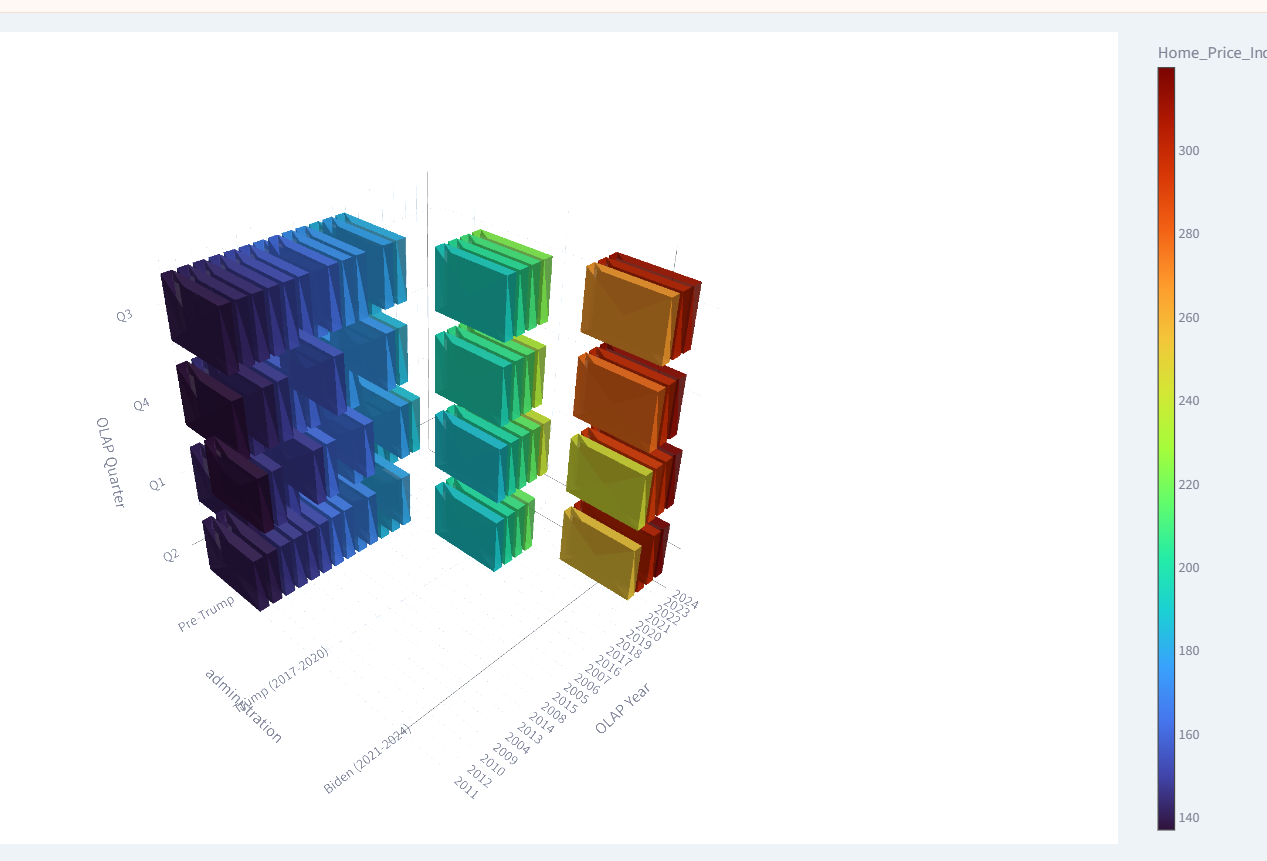
\includegraphics[height=0.78\textheight]{app_screenshots/app_olap.png}
\end{frame}

\begin{frame}{Paper Review Page}
\begin{columns}
\column{0.62\textwidth}
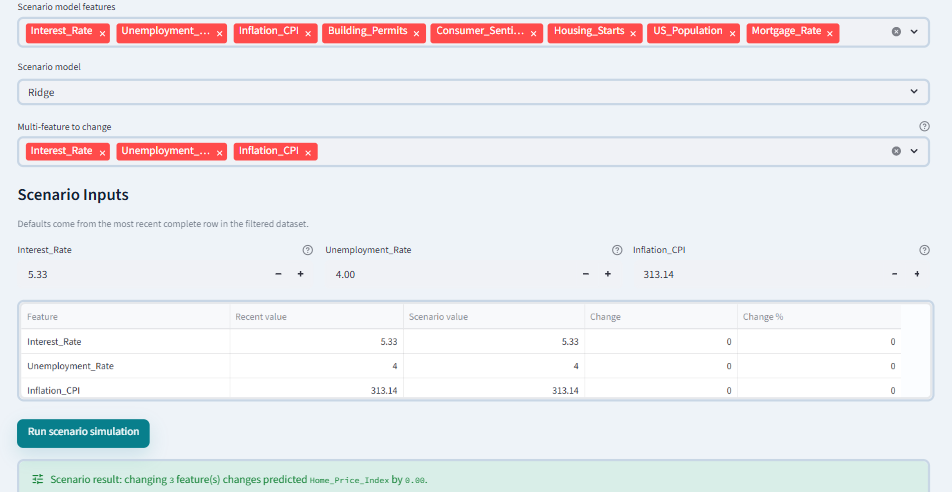
\includegraphics[width=\textwidth]{app_screenshots/app_paper_review.png}
\column{0.36\textwidth}
\begin{itemize}
  \item Links app evidence to housing theory.
  \item Compares results with market context.
  \item Supports a balanced conclusion.
  \item Shows that the project is not only technical.
\end{itemize}
\end{columns}
\end{frame}

\begin{frame}{Production And Governance Page}
\centering
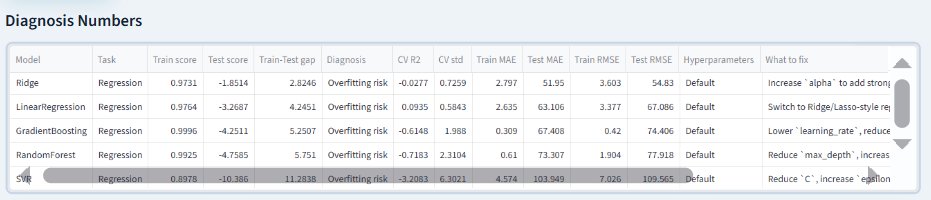
\includegraphics[height=0.78\textheight]{app_screenshots/app_governance.png}
\end{frame}

\begin{frame}{Correlation Results}
\begin{columns}
\column{0.56\textwidth}
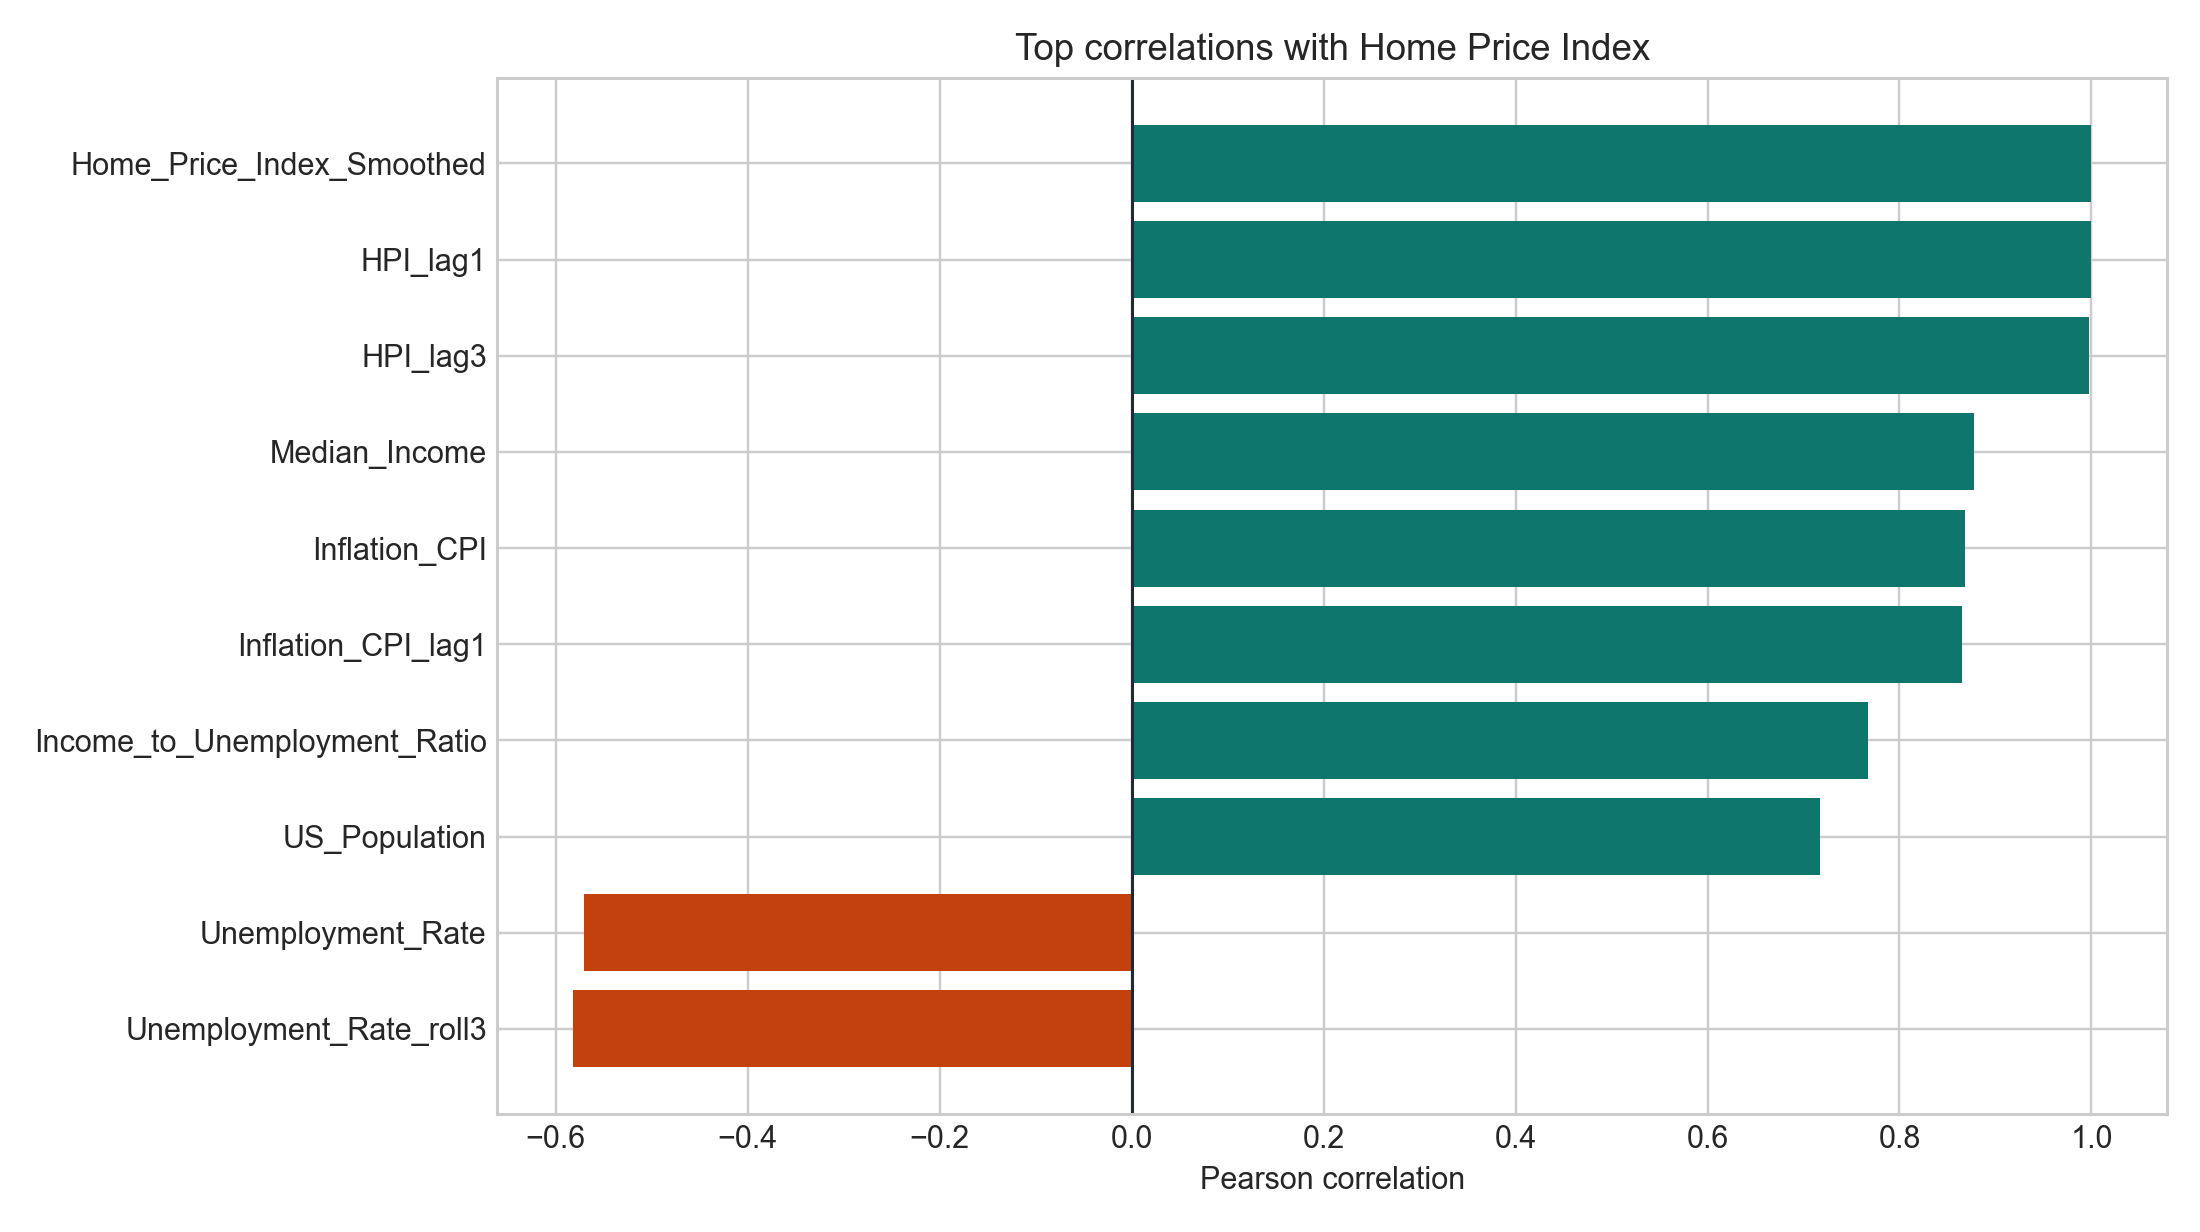
\includegraphics[width=\textwidth]{figures/correlation_results.png}
\column{0.42\textwidth}
\begin{itemize}
  \item Lagged and smoothed price variables are the strongest predictors.
  \item Median income also shows a strong positive relationship with home prices.
  \item Correlation helps guide interpretation but does not prove causality.
  \item The result supports a multi-factor housing-market explanation.
\end{itemize}
\end{columns}
\end{frame}

\begin{frame}{Model Evaluation Results}
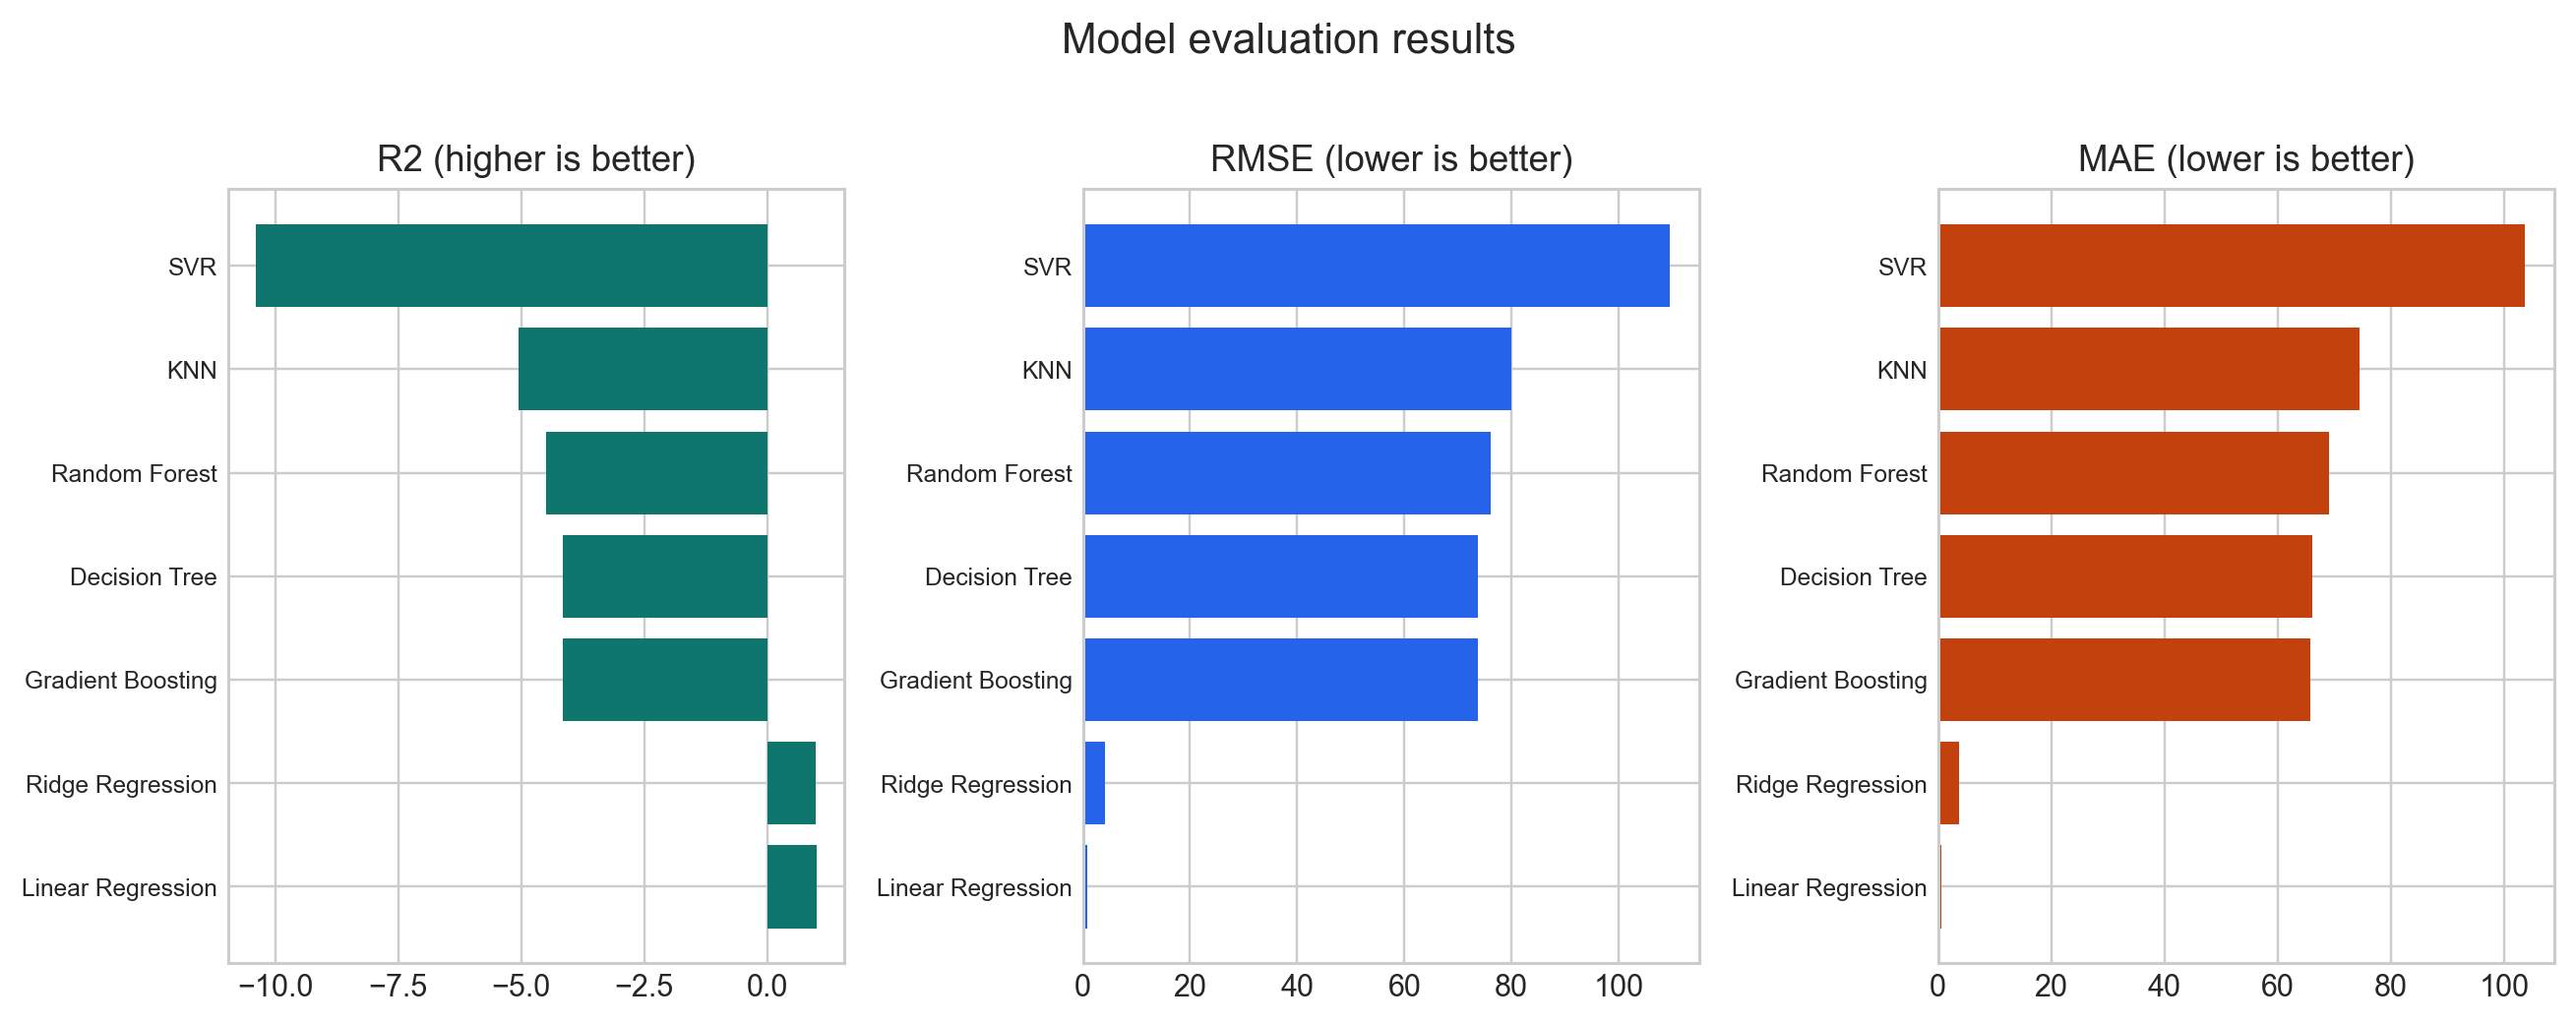
\includegraphics[width=\textwidth]{figures/model_evaluation_results.png}
\vspace{0.4em}
\begin{itemize}
  \item Best generated test result: Linear Regression with \(R^2 = 0.999\), RMSE \(=0.797\), and MAE \(=0.661\).
  \item This result is linked to lagged and smoothed features that preserve the rising trend.
\end{itemize}
\end{frame}

\begin{frame}{Regression Metrics Table}
\begin{center}
\small
\begin{tabular}{lrrrr}
\toprule
Model & MAE & RMSE & \(R^2\) & CV \(R^2\) \\
\midrule
Linear Regression & 0.661 & 0.797 & 0.999 & 0.994 \\
Ridge Regression & 3.715 & 4.162 & 0.984 & -3.135 \\
Gradient Boosting & 65.816 & 73.669 & -4.148 & -2.458 \\
Decision Tree & 66.218 & 73.750 & -4.159 & -3.315 \\
Random Forest & 69.077 & 76.105 & -4.494 & -2.619 \\
KNN & 74.459 & 79.883 & -5.053 & -4.314 \\
SVR & 103.767 & 109.606 & -10.395 & -7.678 \\
\bottomrule
\end{tabular}
\end{center}
\end{frame}

\begin{frame}{Fit Diagnostics}
\begin{columns}
\column{0.57\textwidth}
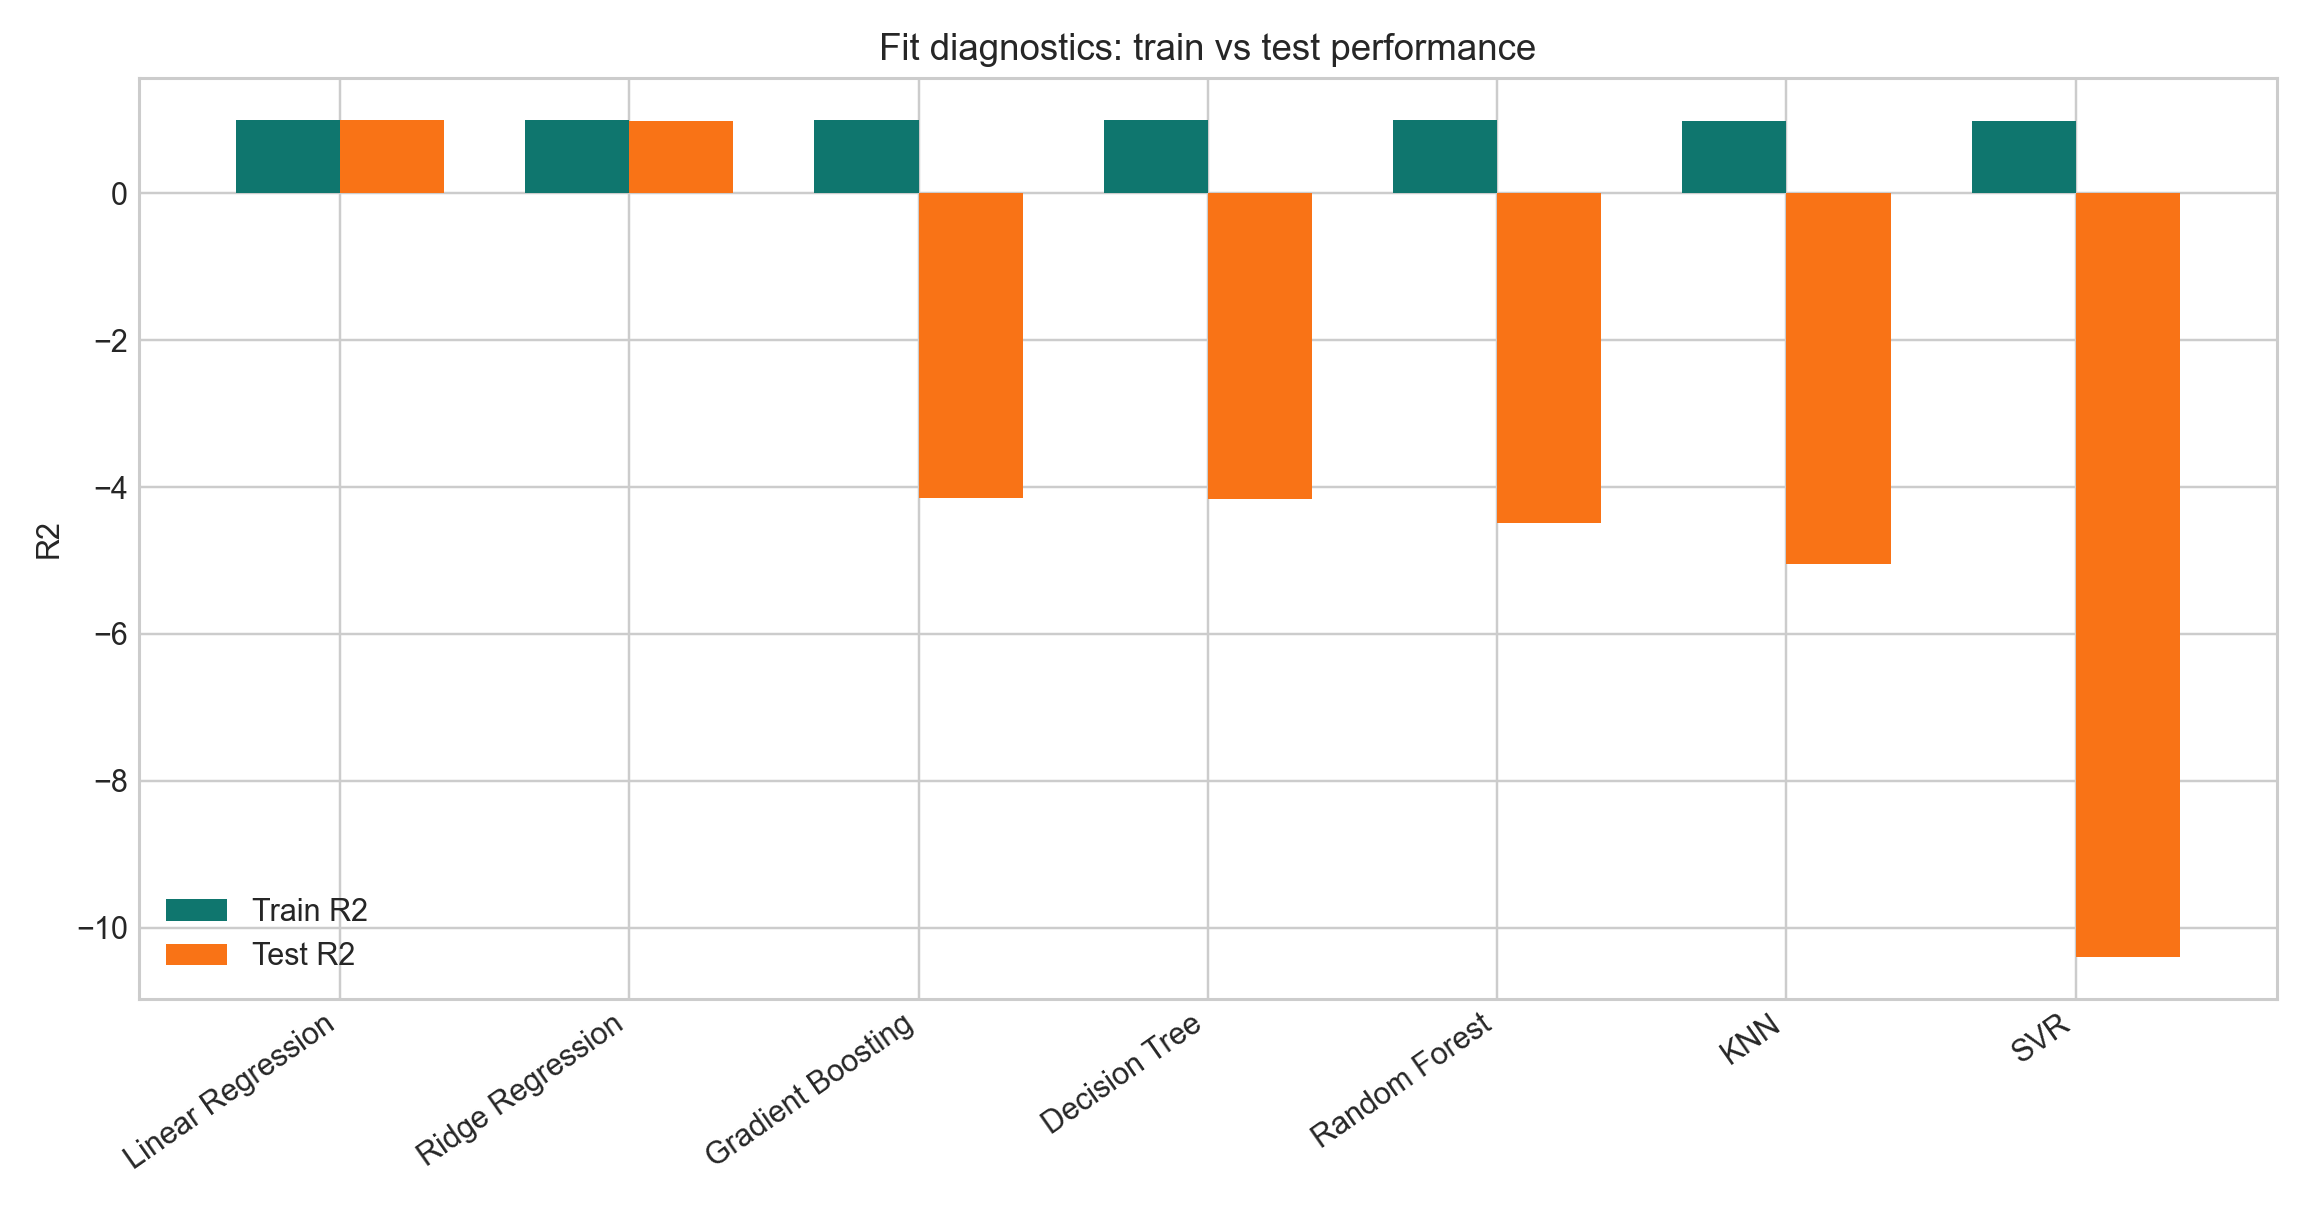
\includegraphics[width=\textwidth]{figures/fit_diagnostics_results.png}
\column{0.41\textwidth}
\begin{itemize}
  \item Diagnostics compare train and test behavior.
  \item Large train-test gaps warn about weak generalization.
  \item Tree-based models struggle when the final test period goes beyond the training range.
  \item A strong report discusses model risk, not only the highest score.
\end{itemize}
\end{columns}
\end{frame}

\begin{frame}{Actual Versus Predicted}
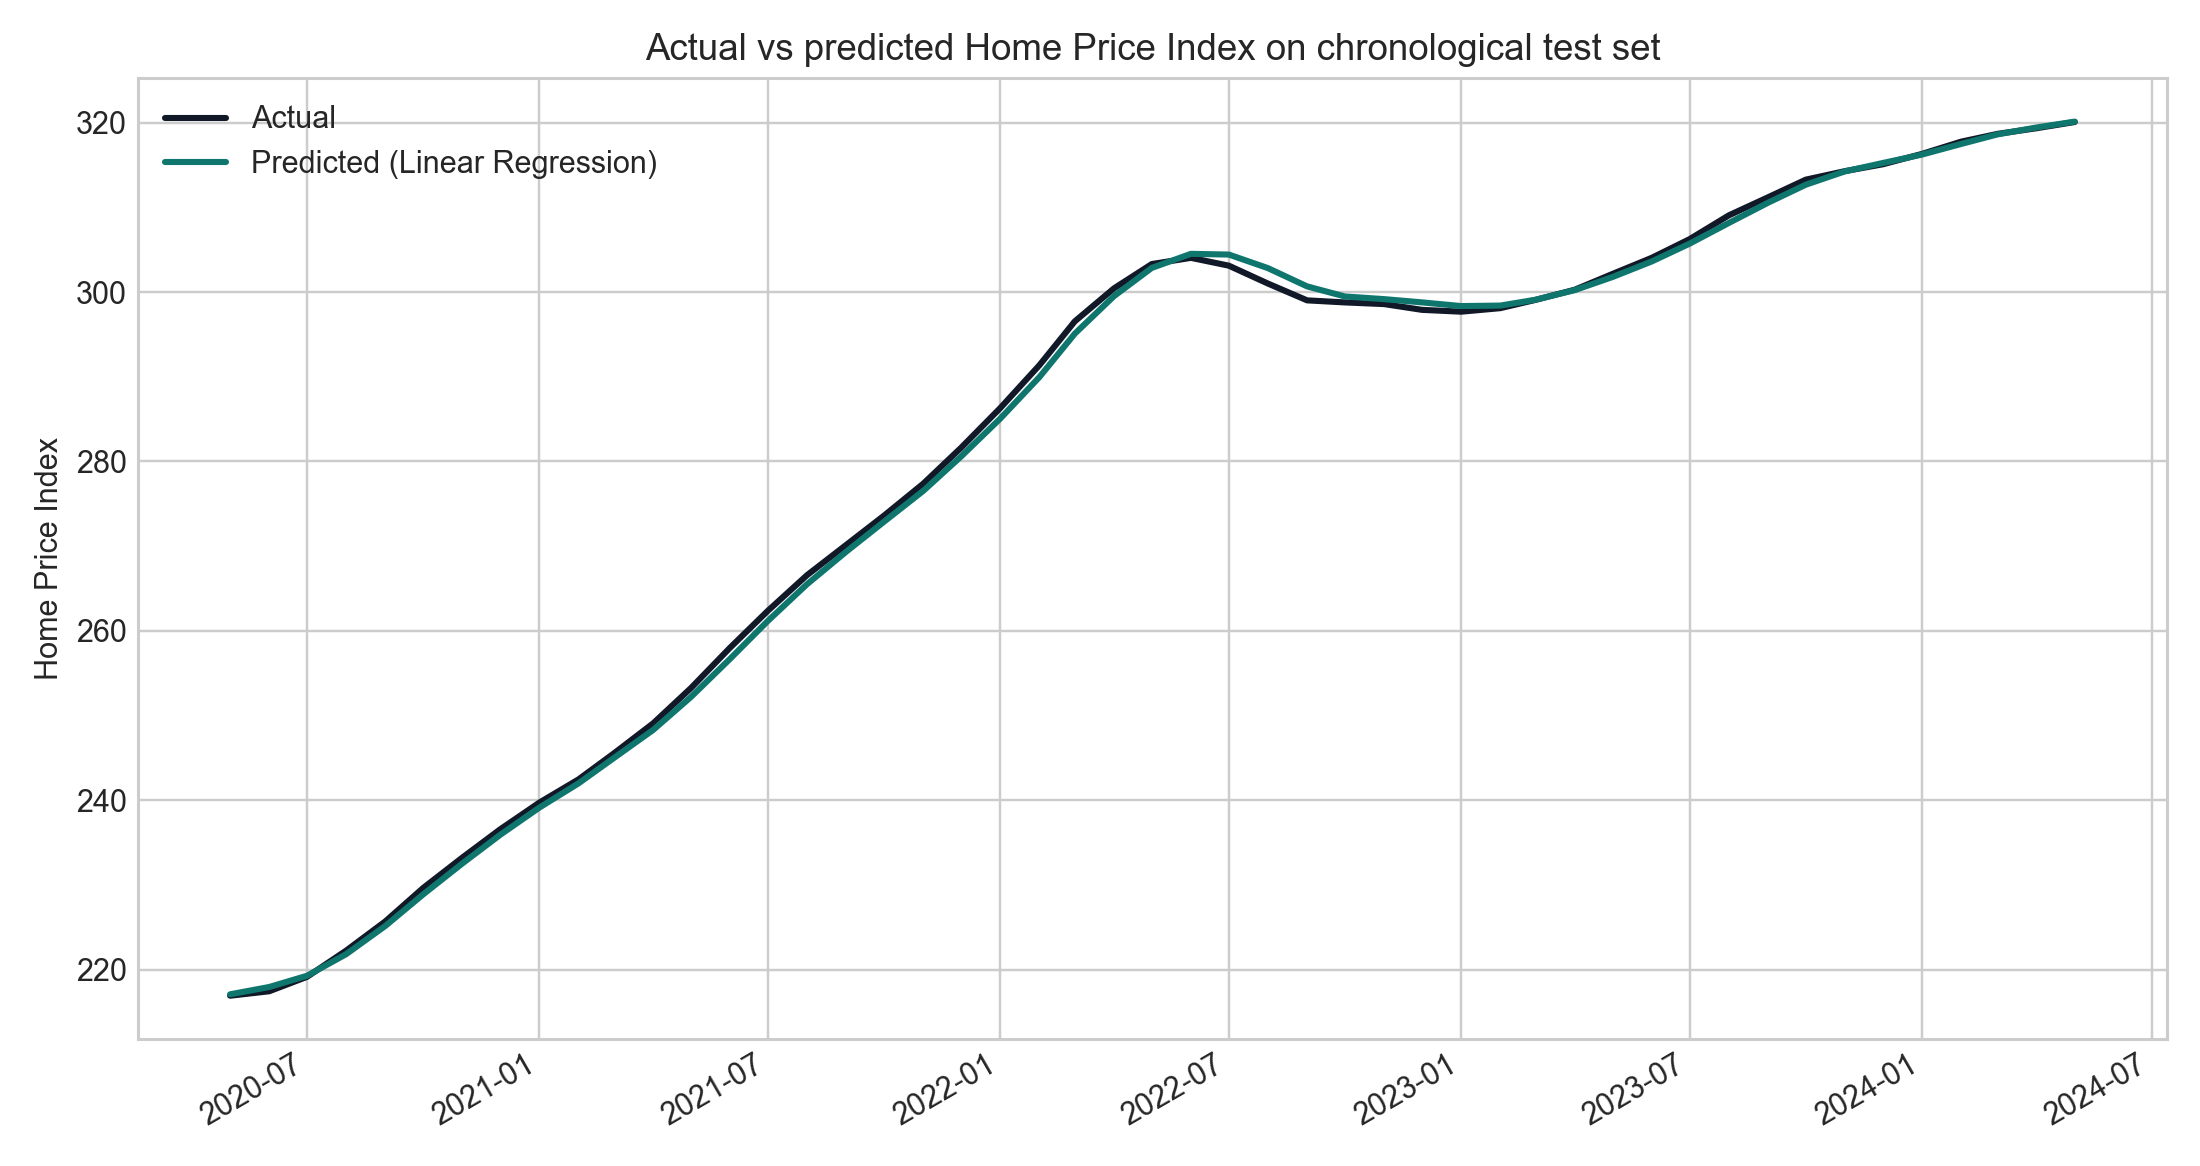
\includegraphics[width=\textwidth]{figures/actual_vs_predicted_results.png}
\begin{itemize}
  \item The best model follows the chronological test period closely.
  \item This supports the predictive value of lagged and smoothed trend features.
\end{itemize}
\end{frame}

\begin{frame}{OLAP Period Results}
\begin{columns}
\column{0.57\textwidth}
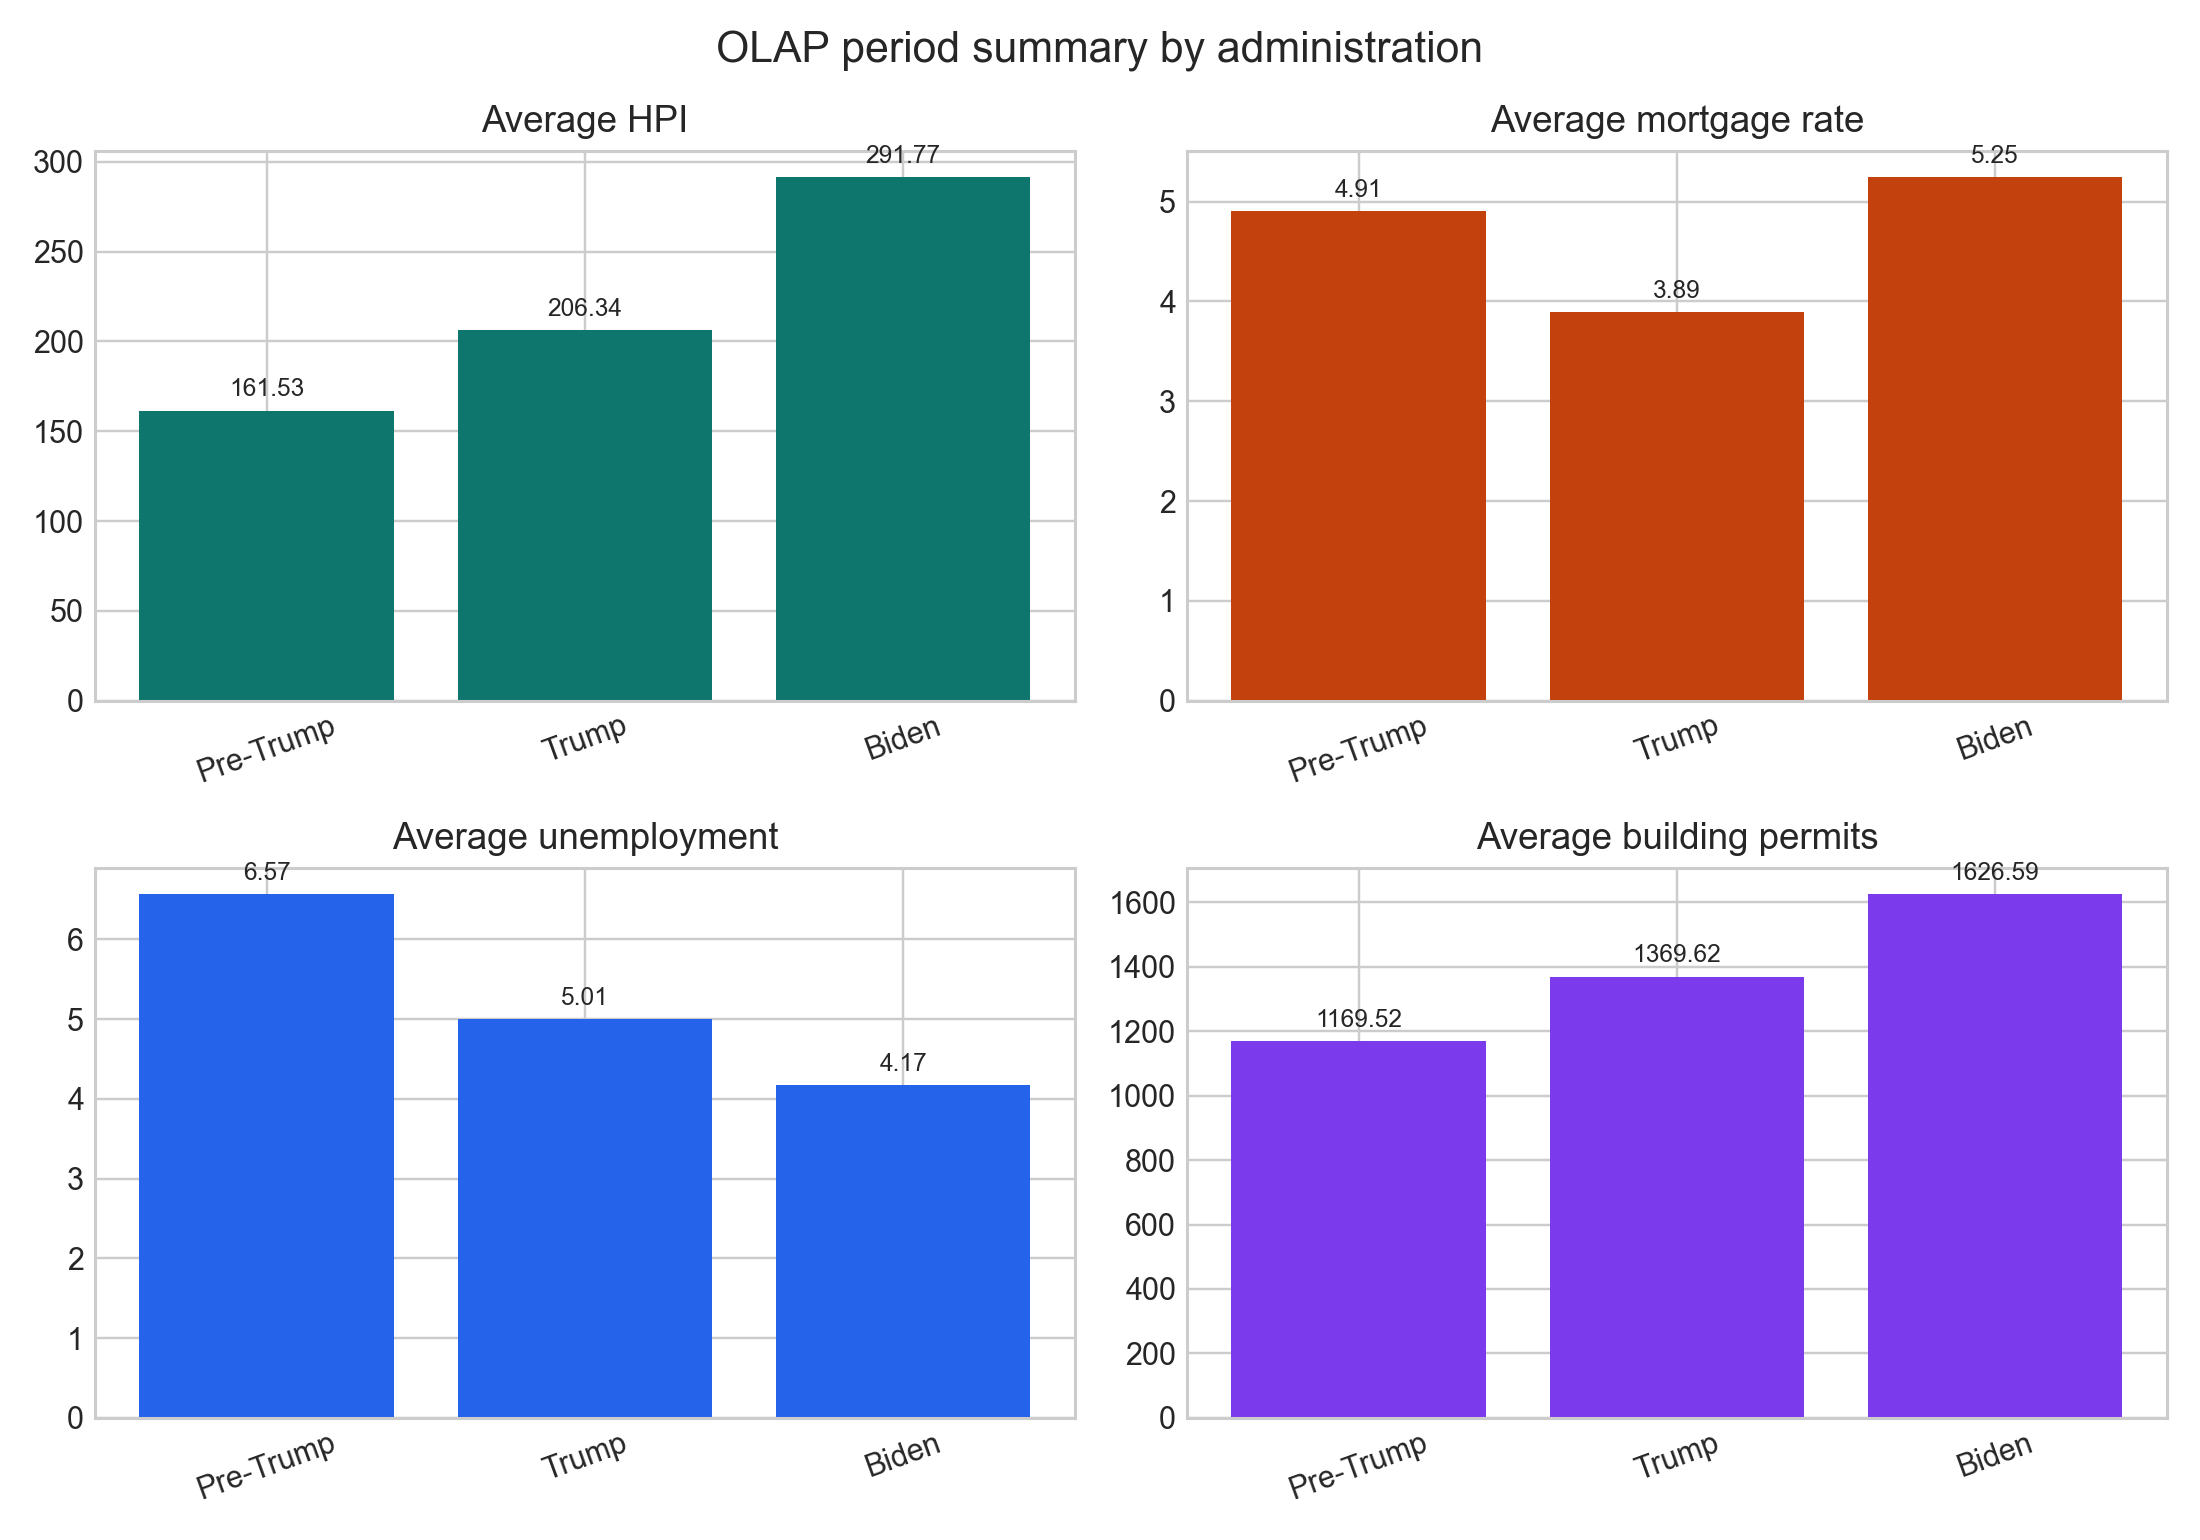
\includegraphics[width=\textwidth]{figures/olap_period_results.png}
\column{0.41\textwidth}
\begin{itemize}
  \item The Biden period has the highest average Home Price Index.
  \item The Biden period also has the highest average mortgage-rate pressure.
  \item This supports the paper-review conclusion that prices and affordability pressure can rise together.
  \item OLAP makes results easier to explain to non-technical users.
\end{itemize}
\end{columns}
\end{frame}

\begin{frame}{Streamlit App Contribution}
\begin{itemize}
  \item Overview and Explore pages show trends, distributions, correlations, and charts.
  \item ML Lab, Evaluation, and Fit Diagnostics compare models and explain performance.
  \item OLAP and Export provide pivot tables, segment stories, 3D cube logic, and CSV downloads.
  \item Paper Review connects dashboard evidence with real-estate theory and current market interpretation.
  \item Production Readiness, Experiment Tracker, and Model Registry introduce governance concepts.
\end{itemize}
\end{frame}

\begin{frame}{Paper Review Message}
\begin{itemize}
  \item Housing prices are shaped by demand, financing conditions, supply, construction, income, and timing.
  \item Higher mortgage rates can reduce affordability, but prices may react slowly when supply remains tight.
  \item The app checks theory using correlations, model evaluation, OLAP segments, diagnostics, and real-market context.
  \item The strongest conclusion is balanced: no single variable explains the housing market alone.
\end{itemize}
\end{frame}

\begin{frame}{Business Impact}
\begin{itemize}
  \item \textbf{Analytical impact:} users can understand which indicators move with housing prices.
  \item \textbf{Decision-support impact:} users can compare models, periods, OLAP segments, and scenarios.
  \item \textbf{Educational impact:} the app demonstrates EDA, supervised learning, unsupervised learning, forecasting, OLAP, and governance in one project.
  \item \textbf{Communication impact:} report graphics and app screenshots make the final defense easier to explain.
\end{itemize}
\end{frame}

\begin{frame}{Limitations And Future Work}
\begin{itemize}
  \item National-level data can hide regional differences between states and cities.
  \item Forecasts remain educational and should not be treated as financial advice.
  \item Future work should add regional datasets, live economic APIs, SHAP explainability, and better chatbot grounding.
  \item A production version should include authentication, monitoring, model drift checks, and persistent experiment storage.
\end{itemize}
\end{frame}

\begin{frame}{Final Conclusion}
\begin{itemize}
  \item The final project is strongest when the report, poster, and app tell one consistent story.
  \item U.S. housing prices require multiple evidence sources: theory, correlations, model evaluation, diagnostics, OLAP, and current context.
  \item The Streamlit dashboard turns the work into a housing intelligence platform, not only a set of charts.
  \item The generated graphics make the final defense more concrete and easier to explain.
\end{itemize}
\end{frame}

\end{document}
